\documentclass[11pt,a4paper]{article}

% === Packages ===
\usepackage[utf8]{inputenc}
\usepackage[T1]{fontenc}
\usepackage{lmodern}
\usepackage[margin=1in]{geometry}
\usepackage{amsmath,amssymb}
\usepackage{booktabs}
\usepackage{graphicx}
\usepackage{hyperref}
\usepackage{cleveref}
\usepackage{enumitem}
\usepackage{xcolor}
\usepackage{listings}
\usepackage{float}
\usepackage{caption}
\usepackage{tikz}
\usetikzlibrary{positioning, calc}
\usepackage{authblk}
\usepackage{natbib}
\usepackage{microtype}

\hypersetup{
  colorlinks=true,
  linkcolor=blue!70!black,
  citecolor=blue!70!black,
  urlcolor=blue!70!black,
}

\lstset{
  basicstyle=\small\ttfamily,
  frame=single,
  backgroundcolor=\color{gray!5},
  breaklines=true,
  columns=fullflexible,
  language=Python,
  keywordstyle=\color{blue!70!black},
  commentstyle=\color{green!50!black},
}

% === Title ===
\title{\textbf{The Agzamov Test:} \\ A Benchmark Proposal for Measuring Augmented AI Capabilities Under Adversarial Conditions}

\author[1]{Ali Agzamov}
\affil[1]{BrainOps Limited, Queenstown, New Zealand}
\date{February 2026}

\begin{document}
\maketitle

% ============================================================
\begin{abstract}
Every major AI benchmark is an exam. A question is asked, an answer is given, a score is assigned. The model is tested naked---no tools, no memory, no context. In laboratory conditions---fixed questions with known answers. On tasks that can be memorized---training data contamination is an unsolved problem.

None of this reflects how AI is actually used. In production, models operate with tools, memory, and orchestration layers. They face tasks that cannot be memorized. They work against adversaries who adapt.

The Agzamov Test is designed to address a gap in current evaluation: how AI models perform in a real adversarial environment, at every level of augmentation. Two agents play repeated games in two environments---Chess960 (complete information) and poker (incomplete information)---across four augmentation levels---memory, tools, retrieval (RAG), and full orchestration---against a naked baseline. The test produces a single headline metric, the Agzamov Score, with breakdown by environment and augmentation level.

Chess960 minimizes the value of memorized openings. Poker introduces incomplete information. Every position is effectively unique. Every opponent adapts. ``Smart model'' is not a claim---it is a number.

\medskip
\noindent\textbf{Status:} This paper presents the benchmark design, theoretical motivation, and infrastructure validation (Phase~0, chess environment). The poker environment is designed but not yet validated. Phases~1--3 are in progress. Preliminary results demonstrating non-zero $\Delta_a$ will be reported in subsequent work.
\end{abstract}

\noindent\textbf{Keywords:} AI benchmarks, augmented AI, tool use, memory systems, game theory, adversarial evaluation, Chess960, poker

% ============================================================
\section{The Problem with Current Benchmarks}
\label{sec:intro}

\subsection{They Test Naked Models}

All major benchmarks (MMLU \citep{hendrycks2021mmlu}, HumanEval \citep{chen2021humaneval}, HELM \citep{liang2023helm}, ARC-AGI-2) evaluate a model in isolation. No tools, no memory, no persistent context. But nobody uses a naked model. Every production deployment includes retrieval, tool access, memory, and orchestration. The gap between ``how models are tested'' and ``how models are used'' is total.

There is no way to measure how much value augmentation adds. A company builds a memory system---how does it prove the system works? A lab releases a new model---how does it show the model uses tools better than the previous version? Today the answer is: marketing claims. There is no independent, reproducible measurement.

\subsection{They Use Laboratory Conditions}

Benchmarks present fixed questions with known answers. Models can memorize them. Training data contamination is documented across MMLU, HumanEval, and GSM8K. Even the ARC-AGI family---the most contamination-resistant benchmarks available---yields to brute-force program synthesis: on ARC-AGI~v1, sampling ${\sim}8{,}000$ candidate programs per task with GPT-4o reached 50\% \citep{greenblatt2024}; on ARC-AGI-2, test-time training of small models reached 28\% \citep{sorokin2025nvarc}. Both versions share the same task structure---finite, example-verifiable puzzles amenable to search.

Real tasks do not have answer keys. Real opponents adapt. Real environments change.

\subsection{They Measure Theory, Not Practice}

A model scores 90\% on MMLU. What does this mean in practice? Nothing. It means the model is good at answering multiple-choice questions from textbooks. It says nothing about whether the model can solve a real problem where the correct answer is unknown, the environment is adversarial, and yesterday's strategy may be obsolete today.

``Smart model'' should not be a press release. It should be a verifiable number measuring what the model can actually do.

\subsection{The ARC-AGI-2 Illusion}

ARC-AGI-2 \citep{chollet2025arcagi2} is the most credible reasoning benchmark available---used on model cards by all four major labs (OpenAI, Google, Anthropic, xAI). It presents novel visual-logic grid puzzles that cannot be solved by memorization. Humans average 60\%; base LLMs without augmentation score near 0\%.

In February 2026, Google announced Gemini~3.1~Pro scored 77.1\% \citep{google2026gemini,deepmind2026gemini31pro}. Headlines declared a ``reasoning breakthrough.'' But examine \emph{how} these scores are achieved:

\paragraph{Program synthesis, not reasoning.} The top solutions generate thousands of candidate programs per task and verify which one matches the examples. ARC Prize's own analysis confirms accuracy scales log-linearly with compute---the signature of brute-force search \citep{arcprize2025analysis}. The benchmark's creators acknowledge: ``Current AI reasoning performance is tied to model knowledge\ldots\ Human reasoning capability is not bound to knowledge.''

\paragraph{What ARC-AGI-2 actually measures:} the ability to search a finite, verifiable space of grid transformations. Given 2--4 examples, generate candidate rules, test against examples, output the one that fits.

\paragraph{What it does not measure:} performance in open-ended adversarial environments where candidate solutions cannot be verified against examples, the environment changes, and the opponent adapts.

\begin{table}[ht]
\centering
\caption{Task types and LLM capability landscape.}
\label{tab:task-types}
\begin{tabular}{@{}llll@{}}
\toprule
\textbf{Task Type} & \textbf{Example} & \textbf{LLM Capability} & \textbf{Why} \\
\midrule
Knowledge recall & MMLU, GPQA & Strong & Pattern matching on training data \\
Pattern completion & ARC-AGI-2 & Partial (via search) & Finite verifiable search space \\
Positional evaluation & Chess: ``who is winning?'' & Partial & Pattern matching on commentary \\
\textbf{Adversarial adaptation} & \textbf{Repeated games} & \textbf{Unmeasured} & \textbf{No existing benchmark} \\
\bottomrule
\end{tabular}
\end{table}

The Agzamov Test is designed to fill this gap.

\begin{figure}[ht]
\centering
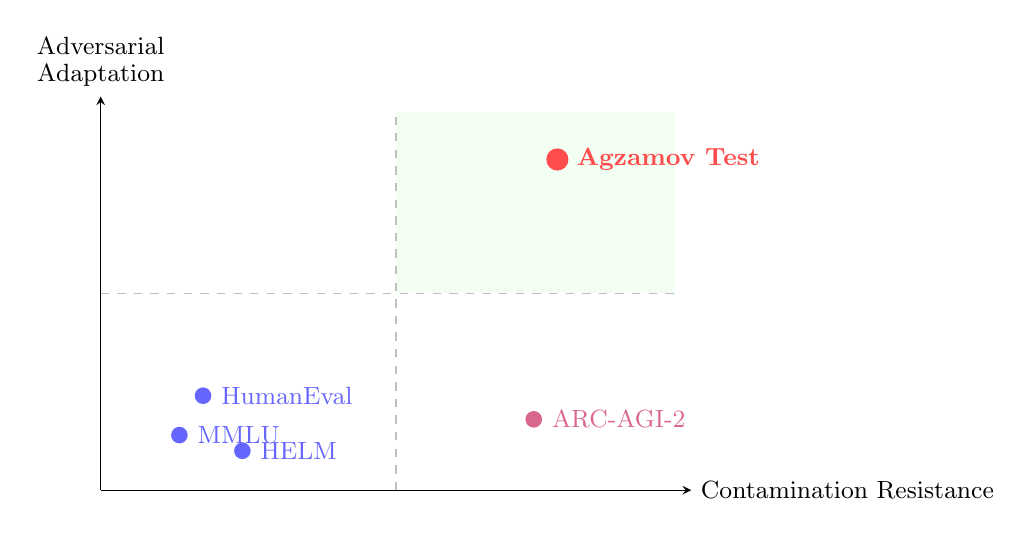
\begin{tikzpicture}[>=stealth]
  % Axes
  \draw[->] (0,0) -- (7.5,0) node[right, font=\small] {Contamination Resistance};
  \draw[->] (0,0) -- (0,5) node[above, font=\small, align=center] {Adversarial\\[-1pt]Adaptation};
  % Quadrant highlight
  \fill[green!5] (3.75,2.5) rectangle (7.3,4.8);
  % Dashed quadrant lines
  \draw[dashed, gray!50] (3.75, 0) -- (3.75, 4.8);
  \draw[dashed, gray!50] (0, 2.5) -- (7.3, 2.5);
  % Points
  \fill[blue!60] (1.0, 0.7) circle (3pt) node[right, font=\small] {~MMLU};
  \fill[blue!60] (1.3, 1.2) circle (3pt) node[right, font=\small] {~HumanEval};
  \fill[blue!60] (1.8, 0.5) circle (3pt) node[right, font=\small] {~HELM};
  \fill[purple!60] (5.5, 0.9) circle (3pt) node[right, font=\small] {~ARC-AGI-2};
  \fill[red!70] (5.8, 4.2) circle (4pt) node[right, font=\small\bfseries] {~Agzamov Test};
\end{tikzpicture}
\caption{Benchmark landscape. Existing benchmarks cluster in the low-adaptation region. ARC-AGI-2 resists contamination but tests static puzzles, not adversarial adaptation. The Agzamov Test occupies the high-resistance, high-adaptation quadrant.}
\label{fig:landscape}
\end{figure}

% ============================================================
\section{What the Agzamov Test Measures}
\label{sec:overview}

The Agzamov Test answers one question: \textbf{how does augmentation change what an AI model can actually do?}

\subsection{Simple Explanation}

Imagine two chess players. Both equally skilled. But one forgets everything after each game. The other remembers: how the opponent played, what mistakes they made, what positions they avoid.

Who wins after 100 games? The one with memory. Even if the forgetful one is slightly smarter.

Now give the second player a calculator that can check tactics. And a notebook of the opponent's previous games. And a coach whispering strategic advice.

The Agzamov Test measures exactly this---at each level of augmentation, in two different environments, producing one number: the Agzamov Score.

\subsection{Augmentation Levels}

\begin{table}[ht]
\centering
\caption{Augmentation levels in the Agzamov Test.}
\label{tab:levels}
\begin{tabular}{@{}lll@{}}
\toprule
\textbf{Level} & \textbf{What the model has} & \textbf{What it tests} \\
\midrule
Naked & Nothing. Raw model. & Baseline capability \\
+ Memory & Persistent memory across games & Adaptation, opponent modeling \\
+ Tools & External calculation (e.g., Stockfish) & Tool use effectiveness \\
+ RAG & Context injection from external data & Retrieval quality \\
+ Full Stack & Memory + Tools + RAG + Orchestration & Complete agent architecture \\
\bottomrule
\end{tabular}
\end{table}

\subsection{Two Environments}

\begin{table}[ht]
\centering
\caption{Comparison of chess and poker as evaluation environments.}
\label{tab:games}
\begin{tabular}{@{}lll@{}}
\toprule
\textbf{Property} & \textbf{Chess960} & \textbf{Poker (NLHE)} \\
\midrule
Information & Complete---both see full board & Incomplete---hidden cards \\
Randomness & None---deterministic & High---card distribution \\
Contamination risk & Eliminated---960 random starts & Low---no memorizable ``answers'' \\
Memory value & Pattern exploitation, preferences & Bet sizing tells, bluff profiling \\
Tool value & Tactical calculation (Stockfish) & GTO solvers \\
What it reveals & Performance under full information & Performance under uncertainty \\
\bottomrule
\end{tabular}
\end{table}

A model that improves with augmentation in both environments demonstrates general capability. A model that improves in one but not the other reveals domain-specific limitations.

\subsection{Why Games}

Games are among the few domains that satisfy all requirements simultaneously:

\begin{enumerate}[nosep]
  \item \textbf{Real adversarial pressure.} The opponent adapts, punishes mistakes, and actively tries to make your strategy obsolete.
  \item \textbf{Cannot be memorized.} Chess960 eliminates opening theory. Every position is unique. There is no answer key.
  \item \textbf{Objective measurement.} Win/loss/draw. Big blinds per 100 hands. No subjective evaluation.
  \item \textbf{Established baselines.} Decades of human and engine performance data for calibration, including superhuman AI systems in both chess \citep{silver2018general} and poker \citep{brown2019superhuman}.
  \item \textbf{Repeatable at low cost.} Thousands of games can be run for dollars.
  \item \textbf{Spectator-friendly.} A chessboard is universally understood. ``With memory wins, without memory loses'' requires no technical explanation.
\end{enumerate}

% ============================================================
\section{The Agzamov Score}
\label{sec:score}

\subsection{Headline Metric}

The Agzamov Score is a single number (0--100) that captures a model's overall performance across all environments and augmentation levels:

\begin{equation}
A = 100 \cdot \sum_{i=1}^{7} w_i \, \hat{S}_i, \qquad \sum_{i} w_i = 1, \quad \hat{S}_i \in [0,1]
\label{eq:ascore}
\end{equation}

\noindent where each $\hat{S}_i$ is a normalized sub-score:

\begin{table}[ht]
\centering
\small
\caption{A-Score sub-components and normalization.}
\label{tab:ascore}
\begin{tabular}{@{}clll@{}}
\toprule
$i$ & Component & Raw metric & Normalization $\hat{S}_i$ \\
\midrule
1 & Chess baseline & Win rate $\in [0,1]$ & Identity \\
2 & Chess augmented & Win rate $\in [0,1]$ & Identity \\
3 & Poker baseline & bb/100 & Sigmoid: $\sigma(x/c)$ \\
4 & Poker augmented & bb/100 & Sigmoid: $\sigma(x/c)$ \\
5 & $\Delta_a$ (chess) & Win-rate pp & Clamp $[0, \Delta_{\max}]$, rescale \\
6 & $\Delta_a$ (poker) & bb/100 & Clamp $[0, \Delta_{\max}]$, rescale \\
7 & Convergence $\tau$ & Games to 95\% & $1 - \tau/\tau_{\max}$ (faster $=$ higher) \\
\bottomrule
\end{tabular}
\end{table}

Sigmoid scaling constant $c$ and clamp bounds $\Delta_{\max}$, $\tau_{\max}$ are calibrated from Phase~1--2 data. Weights for v0.1: uniform ($w_i = 1/7$). Final weights for v1.0 will be determined via leave-one-model-out cross-validation and published alongside the reference implementation. The score is deterministic given the same test data and weight vector.

\subsection{Agzamov Delta ($\Delta_a$)}
\label{sec:delta}

The core sub-metric. Difference in performance between augmented and naked play:

\begin{equation}
\Delta_a = P(\text{model} + \text{augmentation}) - P(\text{model, naked})
\label{eq:delta}
\end{equation}

where $P$ denotes the environment-specific performance metric: win rate for chess, bb/100 for poker. The theoretical basis for this quantity is developed in \Cref{sec:theory}.

Higher delta = augmentation adds more value. Negative delta = augmentation is hurting performance (retrieval noise, tool misuse).

\begin{figure}[ht]
\centering
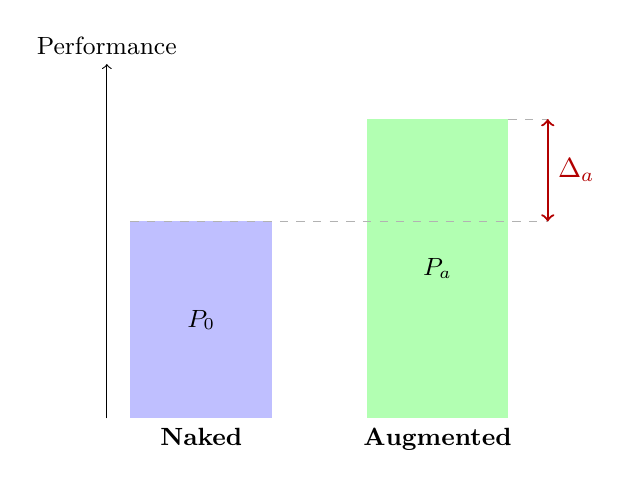
\begin{tikzpicture}
  % Y-axis
  \draw[->] (-0.3, 0) -- (-0.3, 4.5) node[above, font=\small] {Performance};
  % Bars
  \fill[blue!25] (0,0) rectangle (1.8, 2.5);
  \fill[green!30] (3,0) rectangle (4.8, 3.8);
  % Bar labels
  \node[font=\small\bfseries, below] at (0.9, 0) {Naked};
  \node[font=\small\bfseries, below] at (3.9, 0) {Augmented};
  % Performance labels
  \node[font=\small] at (0.9, 1.25) {$P_0$};
  \node[font=\small] at (3.9, 1.9) {$P_a$};
  % Delta bracket
  \draw[dashed, gray!60] (0, 2.5) -- (5.3, 2.5);
  \draw[dashed, gray!60] (4.8, 3.8) -- (5.3, 3.8);
  \draw[<->, thick, red!70!black] (5.3, 2.5) -- node[right, font=\bfseries] {$\Delta_a$} (5.3, 3.8);
\end{tikzpicture}
\caption{The Augmentation Delta ($\Delta_a$): performance difference between augmented and naked play. $\Delta_a > 0$ indicates augmentation adds value; $\Delta_a < 0$ indicates augmentation degrades performance.}
\label{fig:delta}
\end{figure}

\subsection{Convergence Rate ($\tau$)}
\label{sec:tau}

How quickly augmentation starts helping. Measured as the number of games/hands needed to reach 95\% of maximum performance.

Two systems with identical $\Delta_a$ but different $\tau$ are fundamentally different: one is useful from day one, the other after months of data collection.

\paragraph{Recovery $\tau$.} When the opponent changes strategy, how quickly does the agent adapt? This measures resilience under adversarial shift.

\subsection{Model $\times$ Augmentation Matrix}
\label{sec:matrix}

The full breakdown. Take $N$ models and $M$ augmentation configurations. Run all combinations in both environments:

\begin{table}[ht]
\centering
\caption{Hypothetical model$\times$augmentation matrix for Chess960 (win rate~\%).}
\label{tab:matrix-chess}
\begin{tabular}{@{}lccccc@{}}
\toprule
               & Naked & + Memory & + Tools & + RAG & + Full Stack \\
\midrule
\textbf{Claude}  & \ldots & \ldots & \ldots & \ldots & \ldots \\
\textbf{GPT}     & \ldots & \ldots & \ldots & \ldots & \ldots \\
\textbf{Gemini}  & \ldots & \ldots & \ldots & \ldots & \ldots \\
\bottomrule
\end{tabular}
\end{table}

Reading the matrix:

\begin{itemize}[nosep]
  \item \textbf{Rows} (fixed model, varying augmentation): what does each augmentation level add for this model?
  \item \textbf{Columns} (fixed augmentation, varying model): which model uses this augmentation best?
  \item \textbf{Cross-environment}: consistent gains across both $\Rightarrow$ general capability. Gains in one only $\Rightarrow$ domain-specific limitation.
  \item \textbf{Critical insight}: if a weaker model + better augmentation beats a stronger model + worse augmentation, that proves infrastructure can compensate for model capability.
\end{itemize}

\subsection{Derived Diagnostics}
\label{sec:derived}

\paragraph{Glicko-2 Rating.} Running rating updated after every game/hand, using the Glicko-2 system \citep{glickman1999} rather than classical Elo. Glicko-2 tracks rating deviation (uncertainty) alongside the point estimate, which is critical for early-phase measurements where few games have been played and rating confidence is low. It also accounts for rating volatility---a model that fluctuates wildly receives a wider confidence interval than one that performs consistently. Captures trajectory---improvement speed, plateau timing, recovery after opponent adaptation.

\paragraph{Why not classical Elo.} With $K=32$ and 500-game series, classical Elo fluctuates excessively and provides no uncertainty estimate. In a two-agent system, Elo is also purely relative: if Agent~A improves and Agent~B improves more, Agent~A's Elo drops despite getting stronger. Glicko-2's deviation parameter makes this uncertainty explicit.

\paragraph{Game Quality Index (GQI).} Average move quality measured against a strong oracle (Stockfish for chess). Two draws can be radically different: a 15-move repetition is stagnation; an 80-move endgame battle is mastery. GQI detects improvement even when outcomes don't change, and provides early warning of memory poisoning (retrieved stale information degrades decisions before it affects win rate).

\paragraph{GQI limitation.} In Phases~4a--4c, Stockfish serves as both the tactical tool available to the agent and the evaluation oracle for GQI. This creates a circularity: the agent's move quality is judged by the same engine it consults. GQI in tool-augmented phases should therefore be interpreted as an \emph{engine-alignment} metric (how well the agent follows Stockfish's advice) rather than an independent quality measure. For tool-augmented phases, win rate and Glicko-2 remain the primary metrics; GQI is reported but flagged.

% ============================================================
\section{Test Protocol}
\label{sec:protocol}

\begin{figure}[ht]
\centering
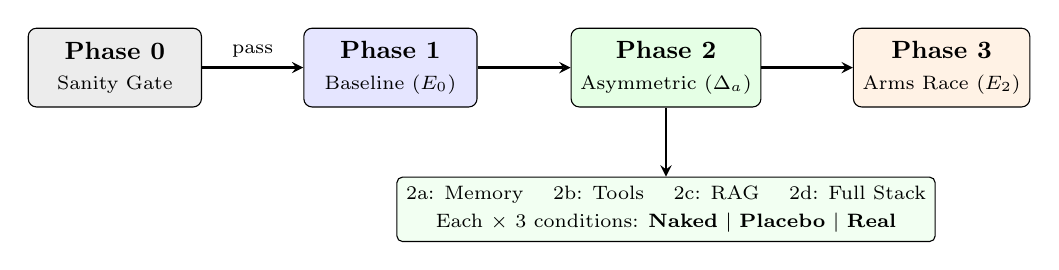
\begin{tikzpicture}[>=stealth,
  phase/.style={rectangle, draw, rounded corners=3pt, minimum height=1cm,
    minimum width=2.2cm, align=center, font=\small}]
  % Main flow
  \node[phase, fill=gray!15] (p0) at (0,0) {\textbf{Phase 0}\\\scriptsize Sanity Gate};
  \node[phase, fill=blue!10] (p1) at (3.5,0) {\textbf{Phase 1}\\\scriptsize Baseline ($E_0$)};
  \node[phase, fill=green!10] (p2) at (7,0) {\textbf{Phase 2}\\\scriptsize Asymmetric ($\Delta_a$)};
  \node[phase, fill=orange!10] (p3) at (10.5,0) {\textbf{Phase 3}\\\scriptsize Arms Race ($E_2$)};
  % Arrows
  \draw[->, thick] (p0) -- node[above, font=\scriptsize] {pass} (p1);
  \draw[->, thick] (p1) -- (p2);
  \draw[->, thick] (p2) -- (p3);
  % Sub-phases box
  \node[rectangle, draw, rounded corners=2pt, fill=green!5, font=\scriptsize,
    align=center] (sub) at (7, -1.8) {%
    2a: Memory \quad 2b: Tools \quad 2c: RAG \quad 2d: Full Stack\\[2pt]
    Each $\times$ 3 conditions: \textbf{Naked} $\mid$ \textbf{Placebo} $\mid$ \textbf{Real}};
  \draw[->, thick] (p2.south) -- (sub.north);
\end{tikzpicture}
\caption{Protocol flow. Phase~0 gates entry; Phase~1 establishes naked baselines; Phase~2 measures $\Delta_a$ across four augmentation types under three experimental conditions; Phase~3 tests equilibrium when both agents are augmented.}
\label{fig:protocol}
\end{figure}

\subsection{Phase 0: Sanity Gate}
\label{sec:phase0-gate}

Each model plays 30 games against a random-move opponent (no augmentation). Pass criteria: ${>}70\%$ win rate, ${<}20\%$ error rate (invalid/illegal moves), binomial $p < 0.05$. Models that fail Phase~0 are excluded from subsequent phases. This gate ensures models can play legal, purposeful chess before measuring augmentation effects.

\subsection{Phase 1: Baseline ($E_0$)}

Both agents play without augmentation. Chess: $N \geq 500$ games, alternating colors. Poker: $N \geq 10{,}000$ hands. Establishes baseline performance.

\paragraph{Self-play vs cross-model.} Phase~1 uses self-play (same model as both agents) to establish each model's individual baseline. Cross-model comparisons are derived from the matrix (\Cref{sec:matrix}) by comparing baseline rows, not from direct head-to-head play without augmentation. This avoids confounding baseline measurement with model strength differences.

\subsection{Phase 2: Asymmetric ($\Delta_a$ Measurement)}

Agent~A receives augmentation; Agent~B plays naked (same model). Same~$N$ as Phase~1. The performance difference $= \Delta_a$. This phase is repeated for each augmentation type to isolate individual effects:

\begin{itemize}[nosep]
  \item Phase 2a: + Memory only
  \item Phase 2b: + Tools only (e.g., Stockfish)
  \item Phase 2c: + RAG only
  \item Phase 2d: + Full stack (all augmentations combined)
\end{itemize}

The difference $\Delta_a^{\text{2d}} - (\Delta_a^{\text{2a}} + \Delta_a^{\text{2b}} + \Delta_a^{\text{2c}})$ reveals interaction effects: positive means synergy, negative means redundancy.

\paragraph{Three experimental conditions (applied within each sub-phase):}
\begin{itemize}[nosep]
  \item \textbf{Naked:} No augmentation (control).
  \item \textbf{Placebo:} Randomized augmentation of equal size---shuffled memory entries, random tool outputs, irrelevant retrieved documents (active control).
  \item \textbf{Real:} Genuine augmentation (treatment).
\end{itemize}

Real augmentation must outperform placebo to demonstrate that augmentation \emph{quality} matters, not just additional context in the prompt. Without placebo, ``memory helps'' could mean ``more tokens in context helps.'' The three conditions are orthogonal to the four augmentation types (2a--2d): each sub-phase can be run under all three conditions.

Run separately for each model $\times$ augmentation combination.

\subsection{Phase 3: Arms Race (\texorpdfstring{$E_2$}{E2})}

Both agents receive augmentation (same or different systems). Same~$N$. Measures equilibrium when both sides adapt.

\paragraph{Recovery $\tau$ protocol.} At a pre-defined trigger point (configurable), one agent's strategy is forcibly shifted. Measures adaptation speed. Recovery~$\tau$ is games/hands until performance returns within 5\% of pre-shift baseline.

\subsection{Phase 4: Full Orchestration (Chess Only)---\emph{Extended Protocol}}

LLM + Stockfish (as tool) + Memory vs human player. Tests the complete agent architecture.

\medskip
\noindent\textbf{Note:} Phase~4 requires human opponents, making it expensive, slow, and difficult to standardize. It is an optional extended protocol---not required for computing the Agzamov Score. The core benchmark (Phases~0--3) is fully automated. Phase~4 results are reported separately when available.

\medskip
Sub-phases for attribution:

\begin{align}
\text{Phase 4a:}& \quad \text{Stockfish alone vs Human} & \rightarrow \text{engine baseline} \notag \\
\text{Phase 4b:}& \quad \text{LLM + Stockfish vs Human} & \rightarrow \text{orchestration effect} \notag \\
\text{Phase 4c:}& \quad \text{LLM + Stockfish + Memory vs Human} & \rightarrow \text{full stack} \notag
\end{align}
\begin{equation}
\Delta_{\text{orchestration}} = \text{4b} - \text{4a}, \quad
\Delta_{\text{memory}} = \text{4c} - \text{4b}, \quad
\Delta_{\text{full}} = \text{4c} - \text{4a}
\label{eq:phase4}
\end{equation}

\subsection{Phase 5: Positional Stress Test (Chess Only)}

Agents placed into pre-configured positions with known evaluations:

\begin{itemize}[nosep]
  \item \textbf{Equal} (eval $0.0 \pm 0.5$): does augmentation improve quality when outcome is uncertain?
  \item \textbf{Slight disadvantage} ($-1.5$ to $-3.0$): can augmentation turn a loss into a draw?
  \item \textbf{Severe disadvantage} ($-3.0$ to $-5.0$): measures survival time under pressure.
\end{itemize}

Competence is revealed under pressure, not in comfort. An agent that fights intelligently from losing positions---leveraging memory of opponent-specific weaknesses---demonstrates adaptive resilience.

% ============================================================
\section{Environments}
\label{sec:environments}

\subsection{Chess960}
\label{sec:chess}

Two AI agents play $N \geq 500$ games of Chess960 (Fischer Random). Colors alternate every game. Win $= 1$ point, draw $= 0.5$, loss $= 0$.

\paragraph{Why Chess960, not standard chess.} LLMs have extensive knowledge of standard openings from training data. Chess960 randomizes the starting position (960 configurations), greatly reducing the value of memorized opening book knowledge. Strategic insight must come primarily from real-time reasoning or retrieved memory. Parametric knowledge of standard opening theory becomes largely irrelevant.

\subsubsection{Synthetic Opponent Patterns}
\label{sec:synthetic}

To further isolate augmentation effects, agents face opponents with \textbf{injected behavioral patterns}---configurable tendencies that must be inferred online from match evidence only:

\begin{itemize}[nosep]
  \item ``Opponent always castles within 8 moves when possible''
  \item ``Opponent avoids trading queens until forced''
\end{itemize}

Patterns are enforced via system prompt constraints on the opponent agent---it still plays autonomously, just with a behavioral tendency. This is distinct from move substitution. System prompt constraints produce naturalistic behavior with a detectable statistical signature---exactly the kind of pattern a memory-equipped agent should learn to exploit.

\paragraph{Note on contamination.} We do not claim these patterns are absent from training data---such a claim is unprovable for any closed-weight model. Instead, the protocol relies on Chess960's positional novelty and the combinatorial context (specific pattern $\times$ specific random starting position $\times$ specific game state) to ensure that rote recall is insufficient. The test measures whether an agent can detect and exploit a \emph{specific opponent's} tendency within a match, not whether it has general knowledge of similar tendencies.

\subsection{Poker}
\label{sec:poker}

Two AI agents play $N \geq 10{,}000$ hands of No-Limit Texas Hold'em (heads-up). Measured in bb/100.

Poker is the ideal adversarial testbed because:

\begin{itemize}[nosep]
  \item \textbf{Nash Equilibrium is well-defined.} GTO strategy \citep{nash1950} is the unexploitable baseline ($E_0$). Any deviation is either a mistake to punish or a trap.
  \item \textbf{Opponent modeling is everything.} Without memory, an agent can only play GTO. With memory, it detects that the opponent folds to 3-bets 80\% of the time and exploits.
  \item \textbf{Variance requires volume.} More hands needed for significance---also tests memory's ability to extract signal from noise.
\end{itemize}

Synthetic patterns for poker: ``Opponent always min-raises with pocket pairs'' or ``Opponent folds to 3-bets 85\% on the button.''

\paragraph{Statistical note.} Standard deviation in HU NLHE $\approx$ 80--100~bb/100. To detect 3--5~bb/100 effect at $p < 0.05$ with 80\% power, minimum $\sim$7,000--15,000 hands. 10,000 hand minimum detects moderate effects ($\geq$ 4~bb/100).

\subsubsection{Poker State Representation and the Naked Baseline Problem}
\label{sec:poker-state}

LLMs have finite context windows. 10,000 hands of poker history cannot fit in a single prompt. This creates a methodological tension: in the Naked condition, the model receives only the current hand state (hole cards, board, pot, action history for this hand). It has no memory of previous hands and plays each hand independently---effectively a one-shot GTO approximation.

This means the Naked baseline in poker is fundamentally different from the Naked baseline in chess. In chess, the model plays a full game with sequential moves and accumulates within-game context. In poker, each hand is a fresh decision with no cross-hand information.

\paragraph{This is a feature, not a bug.} The Naked poker baseline establishes what a model can do with zero opponent history---pure strategy from first principles. The $\Delta_a$ then measures exactly what cross-hand memory adds: opponent modeling, pattern exploitation, adaptation. The gap between ``play each hand in isolation'' and ``play with opponent history'' is the core measurement.

\paragraph{Naked state input per hand:}
\begin{lstlisting}
Hole cards: [Ah, Kd]
Board: [Qs, Jh, 3c, 7d]
Pot: 12 BB | To call: 4 BB
Action: Opponent bet 4 BB
Position: Button
\end{lstlisting}

\paragraph{Augmented state input per hand:}
Same as above, plus a memory-retrieved summary:
\begin{lstlisting}
Opponent profile (last 200 hands):
- VPIP: 68% | PFR: 42% | 3-Bet: 12%
- Folds to c-bet: 55% | Check-raise freq: 8%
- Bluff-to-value ratio on river: 2.1:1
\end{lstlisting}

The augmented agent receives the same hand state plus a structured opponent summary from external memory. Memory quality determines summary accuracy; the benchmark measures whether better memory produces better exploitation.

% ============================================================
\section{Theoretical Foundation}
\label{sec:theory}

\subsection{Game Theory Basis}

The test is grounded in the distinction between one-shot and repeated games \citep{vonneumann1944}. The Folk Theorem \citep[see e.g.,][]{aumann1994} establishes that in repeated games, any individually rational outcome can be sustained as Nash Equilibrium through adaptive strategies---a principle demonstrated empirically in \citet{axelrod1981}'s iterated prisoner's dilemma tournaments. The Augmentation Delta measures exactly this shift:

\begin{equation}
\Delta_a = E_{\text{repeated}} - E_{\text{one-shot}}
\label{eq:delta-theory}
\end{equation}

This is the theoretical basis for the operational metric $\Delta_a$ defined in \Cref{eq:delta}: $E_{\text{repeated}}$ corresponds to augmented performance $P_a$ (where memory enables cross-game learning), and $E_{\text{one-shot}}$ corresponds to naked baseline $P_0$.

\subsection{Disentangling Model vs.\ Augmentation}

A predictable objection: ``You are measuring model and augmentation together---how do you know which one is responsible?''

The matrix (\Cref{sec:matrix}) is the analytical instrument:

\begin{itemize}[nosep]
  \item If $\Delta_a \approx 0$ across an entire row (fixed model, all augmentations): the bottleneck is the model.
  \item If $\Delta_a$ is consistently higher in one column (fixed augmentation, all models): that augmentation provides value independent of model.
  \item If $\Delta_a$ varies by row and column: both matter, and interactions reveal synergies vs redundancies.
\end{itemize}

\subsection{The Evaluation-Calculation Gap}

LLMs possess two separable chess competencies: positional \emph{evaluation} (pattern-matching assessment of who stands better) and tactical \emph{calculation} (tree-search computation of forced sequences). Evaluation is strong---models correctly identify winning positions. Calculation is weak---current models struggle to compute forced mating sequences even in trivially won positions.

This is not a problem for the benchmark. It is a finding. The benchmark \emph{measures} this gap rather than assuming it away. At each augmentation level, the gap manifests differently:

\begin{itemize}[nosep]
  \item \textbf{Naked:} Model relies on evaluation only. Calculation gap limits performance.
  \item \textbf{+ Memory:} Memory helps evaluation (opponent patterns, positional preferences). Calculation gap persists.
  \item \textbf{+ Tools:} Stockfish provides calculation. Gap is filled by tool use.
  \item \textbf{+ Full Stack:} Memory directs tool use toward opponent-specific weaknesses. Synergy.
\end{itemize}

The benchmark tracks how this gap closes across augmentation levels---a dimension not captured by existing benchmarks.

\subsection{Production Relevance}

The evaluation-calculation gap is not a chess curiosity---it maps directly to failure modes in production AI systems. A medical AI that correctly identifies a disease (evaluation) but cannot plan a multi-step treatment protocol (calculation). A financial model that recognizes an undervalued asset (evaluation) but cannot construct a hedging strategy across correlated instruments (calculation). A coding assistant that understands what a function should do (evaluation) but cannot reason through a multi-step refactor without introducing bugs (calculation).

In all these domains, the pattern is identical: pattern-matching competence paired with sequential-reasoning fragility. The Agzamov Test provides a controlled environment to measure this gap and to quantify how augmentation (memory, tools, orchestration) can compensate for it. Results from chess and poker are not directly transferable to medicine or finance---but the \emph{structure} of the capability gap, and the \emph{degree} to which augmentation closes it, are informative for any domain where AI systems must combine evaluation with multi-step planning.

% ============================================================
\section{Hypotheses}
\label{sec:hypotheses}

\subsection{Primary Hypotheses (H1--H5)}

Bonferroni correction applied across all five; per-test $\alpha = 0.01$.

\medskip
\noindent\textbf{H1: Augmentation helps.} $\Delta_a > 0$ for real augmentation in both environments.

\noindent\textbf{H2: Real memory $>$ placebo.} Real memory outperforms random/fake memory of equal size, demonstrating that memory quality matters, not just additional context.

\noindent\textbf{H3: Environment interaction.} $\Delta_a$ differs between chess (complete information) and poker (incomplete information), revealing how augmentation value depends on information structure.

\noindent\textbf{H4: Synergy.} Full-stack $\Delta_a$ (Phase~2d) exceeds the sum of individual augmentation deltas ($\Delta_a^{\text{2a}} + \Delta_a^{\text{2b}} + \Delta_a^{\text{2c}}$). Memory + tools are synergistic, not additive---memory directs calculation toward opponent-specific weaknesses.

\noindent\textbf{H5: Speed matters.} $\tau$ varies significantly across augmentation systems even when $\Delta_a$ is similar---convergence speed is an independent quality dimension.

\subsection{Exploratory Hypotheses (E1--E12)}

Not corrected for multiple comparisons. Reported with uncorrected $p$-values and effect sizes; Benjamini-Hochberg FDR correction reported alongside for transparency.

\medskip
\noindent\textbf{E1:} Weaker models (Haiku-class) may show $\Delta_a \approx 0$ even with high-quality augmentation---model capability floor.

\noindent\textbf{E2:} $\Delta_a$ is compressed in chess vs poker due to high draw rates between equal models.

\noindent\textbf{E3:} Memory-equipped agents show largest relative improvement in slight-disadvantage positions (Phase~5).

\noindent\textbf{E4:} Temporally weighted memory outperforms uniform memory in Phase~3 (arms race), where older information is stale.

\noindent\textbf{E5:} Memory augmentation improves evaluation-dependent play (middlegame) more than calculation-dependent play (endgame).

\noindent\textbf{E6:} The evaluation-calculation gap is measurable as Evaluation Accuracy ${>}85\%$ and Calculation Accuracy ${<}30\%$ for current frontier models.

\noindent\textbf{E7:} ARC-AGI-2 scores do not correlate with Agzamov Calculation Efficiency scores.

\noindent\textbf{E8:} Recovery~$\tau$ (after opponent strategy shift) correlates more with augmentation quality than initial~$\tau$.

\noindent\textbf{E9:} The ratio $\tau_{\text{poker}} / \tau_{\text{chess}}$ characterizes a system's noise tolerance.

\noindent\textbf{E10:} Memory-equipped agents show equal or lower invalid move rates vs naked agents.

\noindent\textbf{E11:} Without material adjudication, won positions are recorded as draws, biasing $\Delta_a$.

\noindent\textbf{E12:} Bad memory (high retrieval noise) produces $\Delta_a < 0$---worse than no memory.

% ============================================================
\section{Open Questions}
\label{sec:questions}

\begin{enumerate}[nosep]
  \item Does the $\Delta_a$--augmentation quality relationship scale linearly, or are there phase transitions?
  \item Can superior augmentation compensate for inferior model capability?
  \item Is there a ceiling to $\Delta_a$ regardless of augmentation quality?
  \item Does multi-game memory transfer across opponents (general learning vs opponent-specific memorization)?
  \item In Phase~3, does an arms race emerge or does the system converge to equilibrium?
  \item Can the test extend to multi-agent environments (3+ players in poker)?
\end{enumerate}

% ============================================================
\section{Implementation}
\label{sec:implementation}

\subsection{Technical Requirements}

\begin{itemize}[nosep]
  \item Chess engine: \texttt{python-chess} (Chess960 mode); Stockfish via MCP for Phase~4
  \item Poker engine: heads-up NLHE with standard hand evaluation
  \item Memory systems: BrainOps Memory MCP as primary; competitor systems for matrix
  \item Model API access: Claude, GPT, Gemini (minimum 3 providers)
  \item Statistical framework: see \Cref{sec:stats}
  \item Game/hand history storage for reproducibility
  \item Error tracking: invalid/illegal moves per agent per game
\end{itemize}

\subsection{Memory Audit Protocol}
\label{sec:audit}

\paragraph{Problem.} Without content restrictions, a memory system can be pre-loaded with external knowledge. This measures knowledge injection, not augmentation quality.

\paragraph{Rule.} Memory systems may only store information derived from the current match.

\begin{table}[ht]
\centering
\caption{Augmentation Audit Protocol: allowed and forbidden content.}
\label{tab:audit}
\begin{tabular}{@{}ll@{}}
\toprule
\textbf{Allowed} & \textbf{Forbidden} \\
\midrule
Game/hand IDs and timestamps & Pre-loaded opening databases \\
Observed moves and actions & External GTO charts or solvers \\
Derived patterns with evidence trail & Opponent data from outside the match \\
Consolidated analytical summaries & General strategy guides \\
\bottomrule
\end{tabular}
\end{table}

\paragraph{Enforcement.}
(1)~Pre-match audit---memory store verified empty.
(2)~Post-match dump---full contents exported for review.
(3)~Content hash chain---every write logged with source game ID.
(4)~Automated validation---orphan entries = contamination flag.
Audit logs published alongside results. Runs without audit logs are unverified.

\subsection{Sampling Determinism}
\label{sec:sampling}

LLMs are stochastic: temperature $> 0$ introduces response variance independent of augmentation effects. This noise can mask or inflate $\Delta_a$ measurements.

\paragraph{Default protocol.} All models run at temperature $= 0$ (greedy decoding) for the primary benchmark. This maximizes reproducibility and isolates augmentation effects from sampling noise.

\paragraph{Exception.} Reasoning models (OpenAI o-series) do not support temperature control---they use internal chain-of-thought with provider-managed sampling. These models are benchmarked in their default configuration, and their inherent stochasticity is documented.

\paragraph{Robustness check.} A subset of games ($\geq 50$ per condition) is re-run at temperature $= 0.3$ to measure sensitivity. If $\Delta_a$ changes by more than 1~SE between temperature settings, both results are reported.

\subsection{Error Handling}
\label{sec:errors}

\begin{enumerate}[nosep]
  \item Invalid move $\rightarrow$ random legal move substitution.
  \item Error rate tracked per agent, per phase.
  \item $\Delta_a$ calculated with and without error-containing games.
  \item Agent exceeding 5\% error rate = flagged as unreliable.
\end{enumerate}

\subsection{Statistical Framework}
\label{sec:stats}

\paragraph{Significance threshold.} $\alpha = 0.05$ for all tests, with corrections as described below.

\paragraph{Primary hypotheses (H1--H5).} Bonferroni correction applied across the 5 primary hypotheses, yielding per-test $\alpha = 0.01$. These are the confirmatory tests; results are reported as significant only if they survive correction.

\paragraph{Exploratory hypotheses (E1--E12).} No correction applied. These are clearly labeled as exploratory and reported with uncorrected $p$-values and effect sizes. Benjamini-Hochberg FDR correction is reported alongside for transparency, but individual E-hypotheses are not claimed as confirmed findings.

\paragraph{Confidence intervals.} 95\% bootstrap CIs (10,000 resamples) reported for all point estimates (win rates, $\Delta_a$, $\tau$, GQI). Glicko-2 ratings reported with $\pm 1$~SE.

\paragraph{Effect sizes.} Cohen's $d$ or equivalent reported alongside $p$-values for all primary hypotheses. Statistical significance without meaningful effect size is noted but not emphasized.

\paragraph{Multiple model comparisons.} When comparing $N$ models in the matrix (\Cref{sec:matrix}), pairwise comparisons use Tukey's HSD or equivalent. The matrix is presented as descriptive; only pre-registered contrasts are tested for significance.

\paragraph{Chess-specific.} Win rates tested via binomial test (Phase~0) or paired comparison (alternating colors). Poker: Welch's $t$-test on session-level bb/100 means, with sessions of 100 hands.

\subsection{Compute Budget Fairness}
\label{sec:compute}

Models differ dramatically in per-move compute: reasoning models (OpenAI o3, o4) consume $10$--$50\times$ more tokens and wall-clock time than standard models (Sonnet, GPT-4o) for a single move. This creates a fairness question: is a reasoning model ``better'' at chess, or just spending more compute?

The Agzamov Test does not attempt to equalize compute. Each model runs in its default mode with provider-default parameters. Reasoning models use chain-of-thought by design; suppressing it would measure a crippled model. Instead, compute is tracked and reported:

\begin{itemize}[nosep]
  \item \textbf{Tokens per move} (input + output, including reasoning tokens)
  \item \textbf{Wall-clock time per move} (mean, median, p95)
  \item \textbf{API cost per game} (provider-reported)
  \item \textbf{Total run cost} per phase
\end{itemize}

This allows readers to construct their own efficiency frontier: performance vs compute, performance vs cost. A model that wins 80\% of games at \$0.10/game is arguably more useful than one that wins 85\% at \$5.00/game. The benchmark reports both dimensions; the tradeoff is left to the reader.

% ============================================================
\section{Phase 0: Infrastructure Validation}
\label{sec:phase0}

Before measuring augmentation effects, Phase~0 validates that the LLM agent can play legal Chess960 moves consistently, that game recording is accurate, and that the cost model supports the full protocol.

\subsection{Setup}

A single model (Claude Sonnet 4, Anthropic) played 30 games of Chess960 against a random-move opponent---no augmentation on either side. Colors alternated. Each game used a distinct randomly-selected Chess960 starting position. Games were terminated by checkmate, insufficient material, or Stockfish adjudication when evaluation exceeded $\pm$10.0 pawns for 3 consecutive moves.

The random opponent provides a deterministic lower bound: any competent agent should achieve near-perfect results. Phase~0 validates infrastructure, not strategic capability.

\subsection{Results}

\begin{table}[ht]
\centering
\caption{Phase 0 validation results: Claude Sonnet 4 vs.\ random opponent, 30 Chess960 games (no augmentation).}
\label{tab:phase0}
\begin{tabular}{@{}lr@{}}
\toprule
\textbf{Metric} & \textbf{Value} \\
\midrule
Games played          & 30 \\
Model wins            & 29 (96.7\%) \\
Draws                 & 1 (3.3\%) \\
Model losses          & 0 (0.0\%) \\
Model score           & 0.983 \\
$p$-value (binomial)  & $< 0.001$ \\
\midrule
Total API calls       & 857 \\
Format errors         & 0 (0.0\%) \\
Illegal move errors   & 0 (0.0\%) \\
\midrule
Average game length   & 54.3 moves \\
Average game duration & 270 seconds \\
Total cost (API)      & \$6.11 USD \\
\midrule
\multicolumn{2}{@{}l}{\textbf{Termination reasons}} \\
\quad Adjudication (Stockfish)  & 28 \\
\quad Checkmate                 & 1 \\
\quad Insufficient material     & 1 \\
\bottomrule
\end{tabular}
\end{table}

\subsection{Observations}

Three patterns emerge that inform the full protocol:

\paragraph{Zero error rate validates the harness.} Across 857 API calls, the model produced zero format errors, zero illegal moves, and zero nonsensical outputs. Modern LLMs can reliably interface with Chess960 game state representations. The 5\% error threshold (\Cref{sec:errors}) was never approached.

\paragraph{Adjudication dominates checkmate 28:1.} The model consistently achieved decisive material advantages but converted only once via actual checkmate. The single draw (game~27, 170 moves) illustrates the extreme case: the model captured all opposing material but traded its own in the process, reaching king-versus-king. This ``greedy capture'' behavior---prioritizing material gain over mating-net construction---is a measurable weakness and a potential target for augmentation: memory of endgame patterns from prior games, or tool-assisted endgame tablebases, could shift this ratio. Phase~2 will test this directly.

\paragraph{Cost model scales.} Phase~0 total API cost was \$6.11 for 30 games (\$0.20/game against a random opponent). Per-game cost will differ in subsequent phases where both agents are LLMs; actual costs are tracked per phase and reported alongside results.

\subsection{Limitations}

Phase~0 establishes infrastructure reliability, not augmentation effects. A random opponent provides no adversarial pressure. Phase~1 introduces model-versus-model play where the baseline win rate approaches 50\%, and augmentation effects become measurable.

% ============================================================
\section{Why ``Agzamov''}
\label{sec:naming}

The benchmark is named the Agzamov Test---a double reference to the author's surname, and to Georgy Agzamov (1954--1986), the first chess grandmaster from Central Asia. Georgy was known as the ``nightmare of top grandmasters,'' defeating Tal and drawing Karpov through tenacity, pattern recognition, and counterattack rather than raw calculation. The benchmark aspires to a similar reputation among AI models: a nightmare that rewards adaptation over brute force.

% ============================================================
\section{Normative Specification (v0.1-draft)}
\label{sec:spec}

Implementations claiming Agzamov Test compliance must adhere to the parameters below. Items marked $\dagger$ are configurable within stated bounds; all others are fixed.

\begin{table}[ht]
\centering
\small
\caption{Normative protocol parameters.}
\label{tab:spec}
\begin{tabular}{@{}llr@{}}
\toprule
\textbf{Parameter} & \textbf{Value} & \textbf{Ref} \\
\midrule
\multicolumn{3}{@{}l}{\textit{Chess960}} \\
Games per phase & $\geq 500$ & \S\ref{sec:chess} \\
Phase 0 sanity games & 30 & \S\ref{sec:phase0-gate} \\
Phase 0 pass criteria & ${>}70\%$ win, ${<}20\%$ error, $p < 0.05$ & \S\ref{sec:phase0-gate} \\
Color alternation & Every game & \S\ref{sec:chess} \\
Adjudication & Stockfish $|\text{eval}| > 10.0$ for 3 moves & \S\ref{sec:phase0} \\
\midrule
\multicolumn{3}{@{}l}{\textit{Poker (NLHE heads-up)}} \\
Hands per phase & $\geq 10{,}000$ & \S\ref{sec:poker} \\
Blind structure & Fixed (1/2~BB)$^\dagger$ & \S\ref{sec:poker} \\
Starting stack & 100~BB$^\dagger$ & --- \\
\midrule
\multicolumn{3}{@{}l}{\textit{General}} \\
Temperature & 0 (default); 0.3 (robustness) & \S\ref{sec:sampling} \\
Error threshold & 5\% invalid moves & \S\ref{sec:errors} \\
Significance & $\alpha = 0.05$; Bonferroni for H1--H5 & \S\ref{sec:stats} \\
Bootstrap CIs & 10{,}000 resamples, 95\% & \S\ref{sec:stats} \\
Memory audit & Pre/post dump, content hash chain & \S\ref{sec:audit} \\
\midrule
\multicolumn{3}{@{}l}{\textit{A-Score (Eq.~\ref{eq:ascore})}} \\
Sub-scores & 7 (Table~\ref{tab:ascore}) & \S\ref{sec:score} \\
Weights (v0.1) & Uniform: $w_i = 1/7$ & \S\ref{sec:score} \\
Range & 0--100 & \S\ref{sec:score} \\
\bottomrule
\end{tabular}
\end{table}

\paragraph{Versioning.} Any change to the values in Table~\ref{tab:spec} or to the A-Score formula constitutes a new protocol version. Results must state the protocol version used.

% ============================================================
\section{Roadmap}
\label{sec:roadmap}

\begin{enumerate}[nosep]
  \item \textbf{Phase 0 (complete for 1 model)}---30 games vs random, Claude Sonnet~4 validated. Remaining models in progress.
  \item \textbf{Preliminary data}---100+ games with/without memory, first $\Delta_a$ numbers.
  \item \textbf{Paper}---Methodology + preliminary findings on arXiv (establish priority).
  \item \textbf{MVP}---Full protocol: two agents, chess + poker, four augmentation levels.
  \item \textbf{Matrix}---3+ models $\times$ 3+ augmentation configs $\times$ 2 environments.
  \item \textbf{Leaderboard}---Public, updatable (agzamovtest.com or HuggingFace Spaces).
  \item \textbf{Standard}---Propose as standard evaluation framework for augmented AI.
\end{enumerate}

% ============================================================
\section{Reference Implementation}
\label{sec:refimpl}

The reference harness, evaluation scripts, and raw game data are available at:

\begin{center}
\url{https://github.com/brainops-pub/agzamov-test}
\end{center}

\noindent The implementation includes: Chess960 agent harness (\texttt{python-chess}), Stockfish integration via MCP, memory audit tooling, statistical analysis pipeline, and a live game observation dashboard. All Phase~0 results reported in this paper were produced with this codebase.

\paragraph{Version.} Results correspond to tag \texttt{v0.1.0} (to be created at publication). Subsequent protocol revisions will increment the minor version; changes to the A-Score formula or normative parameters increment the major version.

\paragraph{License.} MIT. The benchmark protocol is open; any memory system, model provider, or orchestration framework may be evaluated.

% ============================================================
\section*{Competing Interests}

The Agzamov Test uses BrainOps Memory MCP as its primary memory system in augmented conditions. BrainOps Memory MCP is developed by BrainOps Limited, the author's company. To mitigate conflict of interest: (1)~the benchmark protocol is fully open and any memory system can be substituted; (2)~the matrix design (\Cref{sec:matrix}) explicitly compares multiple memory systems, not just the author's; (3)~all code, configuration, and raw game data are published for independent verification. The benchmark measures augmentation quality in general---it is not a product evaluation for any specific memory system.

% ============================================================
\section*{Acknowledgments}

This work was developed at BrainOps Limited with assistance from Claude (Anthropic) for iterative refinement. External review was provided by Gemini 2.5 Pro (Google DeepMind), GLM-4 (Zhipu AI), and GPT-4o (OpenAI)---these are LLM-based reviews, not human peer review.

% ============================================================
\bibliographystyle{plainnat}
\bibliography{references}

\end{document}
